\section{Конструкторская часть}
В данном разделе будут представлена IDEF0 диаграмма метода, схемы алгоритма и структура приложения. Описан формат входных и выходных данных.

\subsection{IDEF0 диаграмма}
\begin{figure}[h]
	\begin{center}
		{\includegraphics[scale=0.5, angle=-90, page=1]{img/idef0.pdf}}
		\caption{IDEF0 диаграмма, верхний уровень}
		\label{idef0:top}
	\end{center}
\end{figure}

\begin{figure}[h]
	\begin{center}
		{\includegraphics[scale=0.5, angle=-90, page=2]{img/idef0.pdf}}
		\caption{IDEF0 диаграмма, декомпозиция А0}
		\label{idef0:A0}
	\end{center}
\end{figure}

\begin{figure}[h]
	\begin{center}
		{\includegraphics[scale=0.5, angle=-90, page=3]{img/idef0.pdf}}
		\caption{IDEF0 диаграмма, декомпозиция А1}
		\label{idef0:A1}
	\end{center}
\end{figure}

\begin{figure}[h]
	\begin{center}
		{\includegraphics[scale=0.5, angle=-90, page=4]{img/idef0.pdf}}
		\caption{IDEF0 диаграмма, декомпозиция А2}
		\label{idef0:A2}
	\end{center}
\end{figure}

\begin{figure}[h]
	\begin{center}
		{\includegraphics[scale=0.5, angle=-90, page=6]{img/idef0.pdf}}
		\caption{IDEF0 диаграмма, декомпозиция А3}
		\label{idef0:A3}
	\end{center}
\end{figure}

\subsection{Схема алгоритмов}


\begin{figure}[h]
	\begin{center}
		{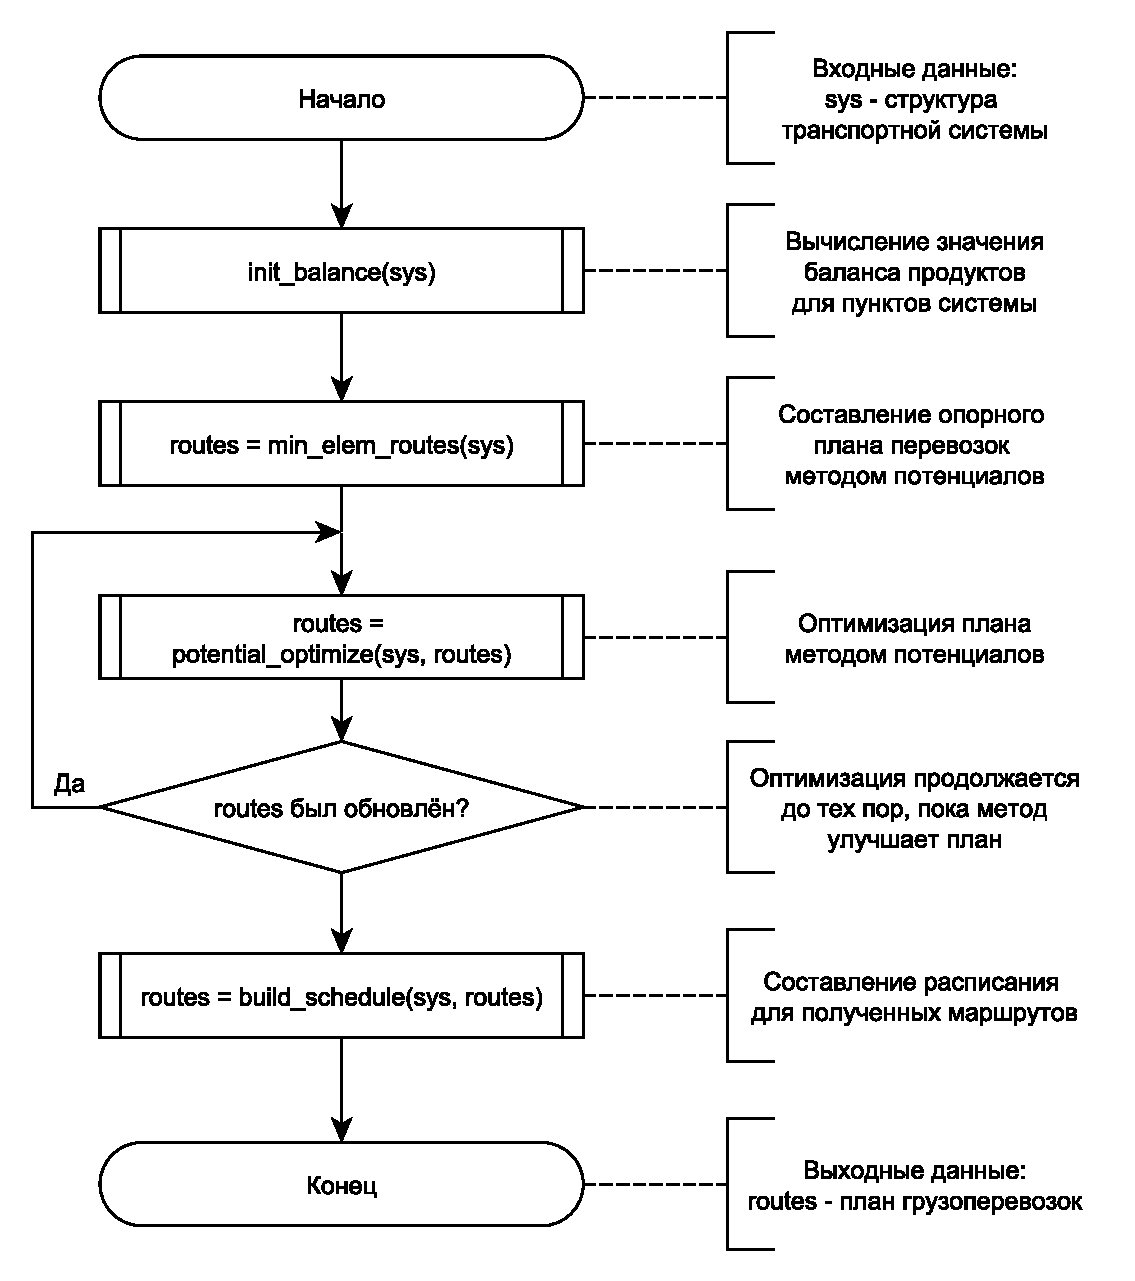
\includegraphics[scale=0.7, angle=0, page=1]{img/main_algorithm.pdf}}
		\caption{Схема общего алгоритма программы}
		\label{alg:main}
	\end{center}
\end{figure}

\pagebreak